% !TeX spellcheck = en_GB
\documentclass[11pt]{article}
\usepackage{graphicx}
\usepackage{listings}
\title{Machine Learning Project\\Task 1}
\author{Duy Nguyen Dinh \\ dinh@rhrk.uni-kl.de\and
	Minh Duc Duong\\ duong@rhrk.uni-kl.de\and
    ---\\ ---}
\date{\today}
\begin{document}

\maketitle

\section{K Nearest Neighbor Classification}

\subsection{Classes of the data set}
First we look into the data set, which will be used to fit the model as well as evaluate the accuracy of the model. The data consists of a total of 15000 images, each one was assigned with a specific label. Here is what each class in the data set looks like:

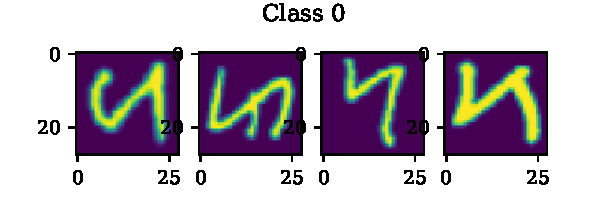
\includegraphics{figures/1a_sample_class_0.pdf}

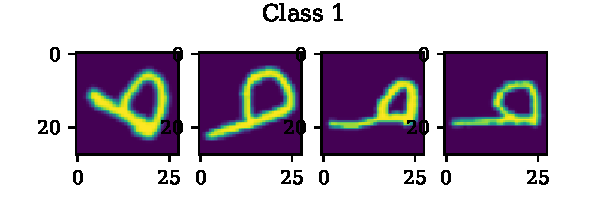
\includegraphics{figures/1a_sample_class_1.pdf}

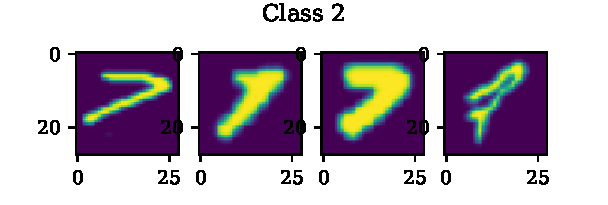
\includegraphics{figures/1a_sample_class_2.pdf}

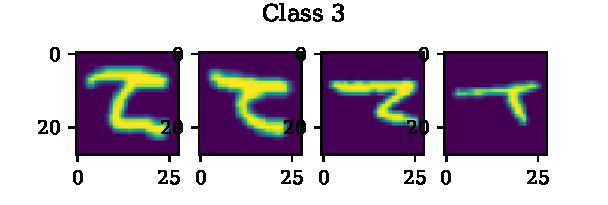
\includegraphics{figures/1a_sample_class_3.pdf}

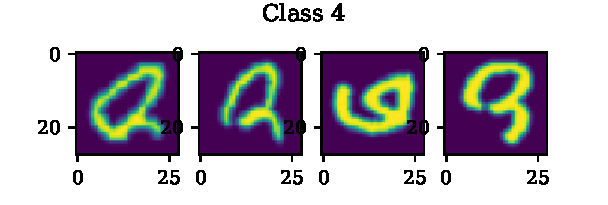
\includegraphics{figures/1a_sample_class_4.pdf}

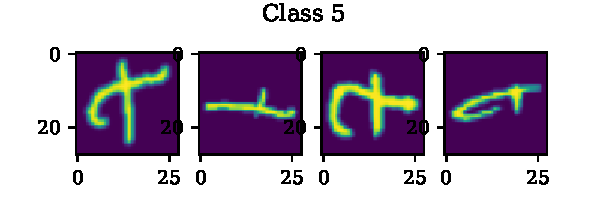
\includegraphics{figures/1a_sample_class_5.pdf}

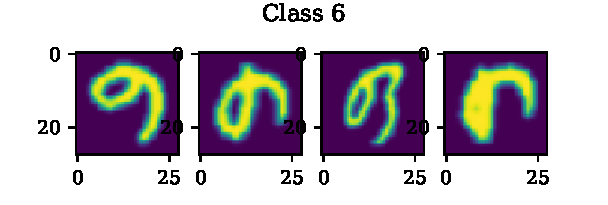
\includegraphics{figures/1a_sample_class_6.pdf}

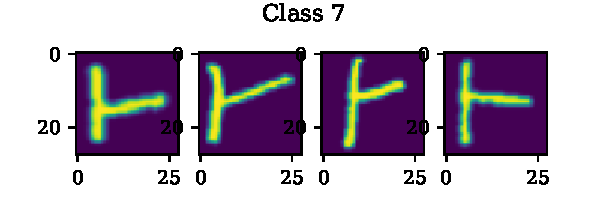
\includegraphics{figures/1a_sample_class_7.pdf}

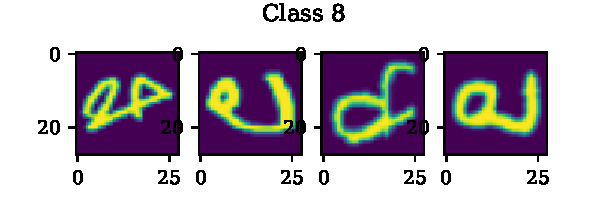
\includegraphics{figures/1a_sample_class_8.pdf}

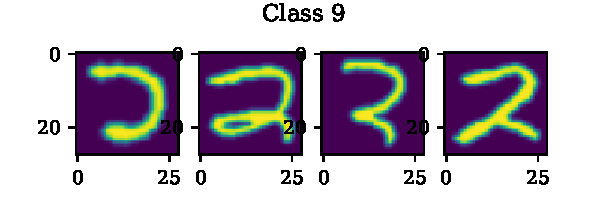
\includegraphics{figures/1a_sample_class_9.pdf}

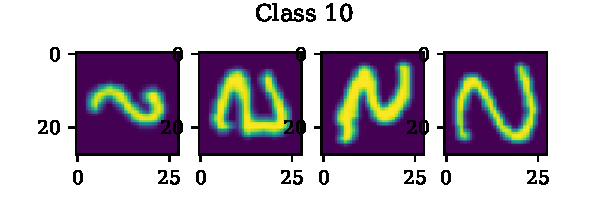
\includegraphics{figures/1a_sample_class_10.pdf}

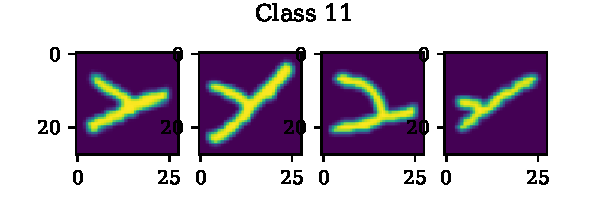
\includegraphics{figures/1a_sample_class_11.pdf}

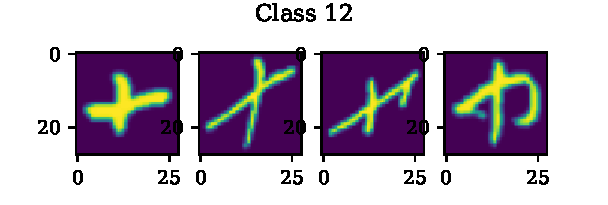
\includegraphics{figures/1a_sample_class_12.pdf}

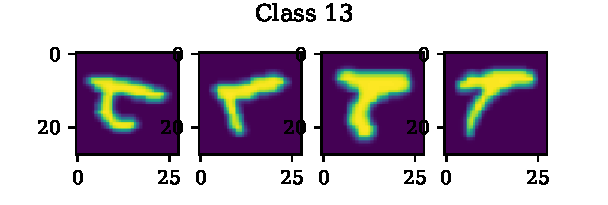
\includegraphics{figures/1a_sample_class_13.pdf}

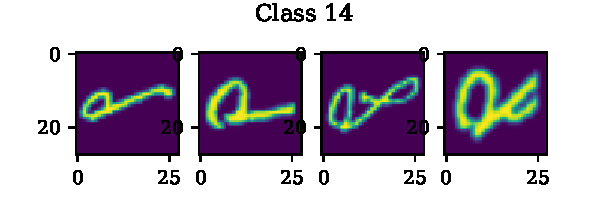
\includegraphics{figures/1a_sample_class_14.pdf}

There are 15 different classes in the data, which was counted from 0 to 14. Each of these classes may have an unique pattern: For example, Images in class 7 look like a letter 'T', which was rotated 90 degree to the left. Images in class 1 look like a letter 'q', which was rotated 90 degree to the right. It is important to note that through normal observation, it can be very challenging to recognize the pattern or the common properties of all images in the same class. Therefore it is necessary to create a classification, which can be used to determine the class of object that can not be done with simple human observation.

\subsection{Implementation of KNN}

A class was implemented to define every KNN-classifier. A classifier has many different properties:
\begin{itemize}
    \item k: The amount of images that we need to identify the label of calculating image
    \item dist\_function: The method to calculate the distance between image
    \item filter: Filter For the calculating image, which is required later into the task
    \item return\_neighbor: Check if we want to save the k-nearest neighbors for each image, which is useful later to identify neighbors of misclassified images
\end{itemize}

\begin{lstlisting}[language=python, caption=KNN class]
class KNN:
    def __init__(self, k=5, dist_function=euclidean_distance
            , filter=None, return_neighbor=False):
        self.k = k
        self.dist_function = dist_function
        self.return_neighbor = return_neighbor
        self.filter = filter

    def fit(self, X, y):
        if self.filter is not None:
            X = np.array([convolve(i, self.filter) for i in X])
        self.train_x = X
        self.train_y = y

    def predict(self, X):
        if self.filter is not None:
            X = np.array([convolve(i, self.filter) for i in X])
        return [knn(x, self.train_x, self.k, self.train_y
                , self.dist_function, self.return_neighbor) for x in X]
\end{lstlisting}


The fit method will get the data as "train data", so we will calculate the distance between the images, which we need to predict the label, with these "train-images". The method predict will call the function knn, which calculate the label for each image in the set. The algorithm of this function was demonstrated in the task sheet and the implementation can be found in knn.py

\subsection{m-fold cross validation on different k}

We implemented m-fold cross validation and the Euclidean distance functions as described in the task sheet. As the sheet required, we run 5 fold cross validation on the entire set of 15000 images with k vary from 1 to 10.

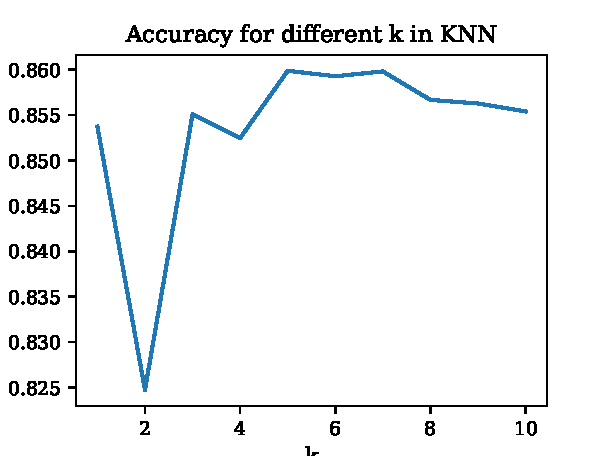
\includegraphics{figures/1c_knn_acc_k.pdf}

The peak of accuracy is achieved with k=5. Therefore all of the classifier will have k=5 from now on.

\subsection{Is the best current k a good choice?}

While it is a good indicator to choose the k, which has the best accuracy at the moment, it may not the best choice to test on new fresh images. As more images will be used to fit the classifier, new images come with many unseen properties or the distribution of classes can be changed. If we use the approach KNN, it should be a good practice to test out on different values of k, especially since k is not the only factor decides the accuracy of the model (for example the amount, quality and distribution of data also matters).

\subsection{KNN with different distance metric}

To improve the speed of the program, we prefer to use built-in functions from Numpy and Scipy to define the distance functions rather than implement it ourself.

\begin{lstlisting}[language=python, caption=distance functions]
def euclidean_distance(a, b):
    return np.linalg.norm(np.squeeze(a - b))

def manhattan_distance(a, b):
    return np.linalg.norm(np.squeeze(a - b), 1)

def minkowki_distance(p, q):
    return distance.minkowski(p.flatten(), q.flatten())
\end{lstlisting}

The Euclidean distance function is a specific case of Minkowski distance function with the scalar of 2. This time we test the accuracy of Euclidean metric compare to Manhattan metric (Minkowski with scalar of 1) and Minkowski metric with scalar of 3.

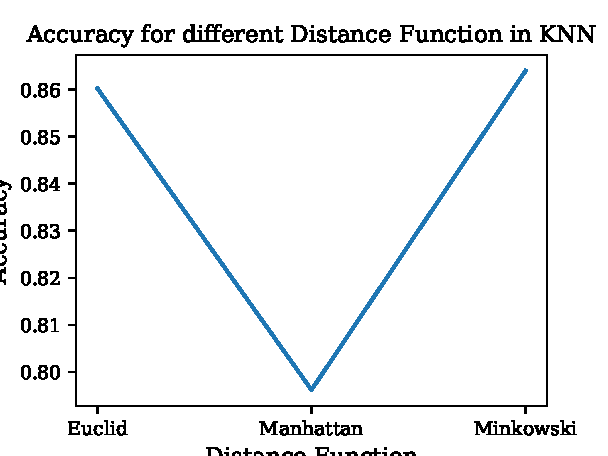
\includegraphics{figures/1e_knn_acc_dist.pdf}

The result shown, the accuracy of Euclidean metric and Minkowski metric are similar and Manhattan metric has a 6\% lower in accuracy.

\subsection{Feature Engineering}

The convolutional operation is implemented as follows. We assume that the images are only in grayscale, the size of the dimension C is 1.

\begin{lstlisting}[language=python, caption=convolve function]
def convolve(x, filter):
    x = np.squeeze(x)
    x_h, x_w = x.shape
    filter = np.flipud(np.fliplr(filter))
    filter_h, filter_w = filter.shape
    res_h = x_h - filter_h + 1
    res_w = x_w - filter_w + 1
    res = np.zeros((res_h, res_w))
    for i in range(res_h):
        for j in range(res_w):
            res[i, j] = (filter * x[i: i + filter_h, j: j + filter_w]).sum()
    return res
\end{lstlisting}

\subsection{Experiment with filters}

With the implemented convolutional operation, we test the classifier in 5 different cases (without filter, blur filter and edge filter, the combination of 2 filter, blur filter with built-in convovle2d function of scipy) using 5-fold cross validation.

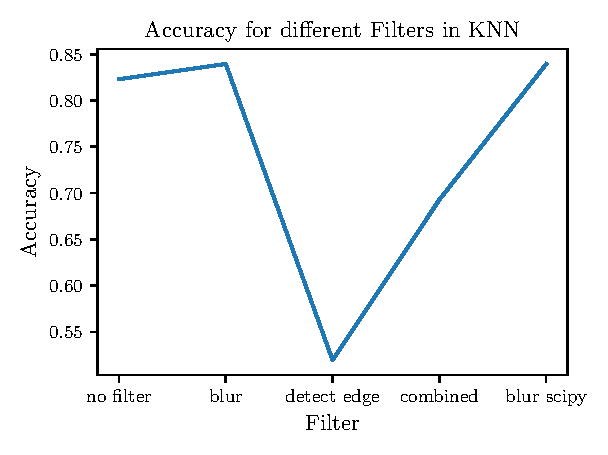
\includegraphics{figures/1g_knn_acc_filter.pdf}

Blur filter improve our KNN-classifier a little while we have a significantly drop in accuracy with edge detection approach. The combination produces an average result of those. The accuracy isn't changed when using built-in convolve2d function from scipy, only that the built-in function is faster.


\subsection{Weight KNN}

Now we assigned weight into each neighbor, which is inversely proportional to the distance. This means the closer the neighbor to the test image, the more impact it will make to the result of the prediction. We modify our knn function with a new added parameter inverse\_modifier to calculate the weight of each neighbor (inverse\_modifier divided by distance)

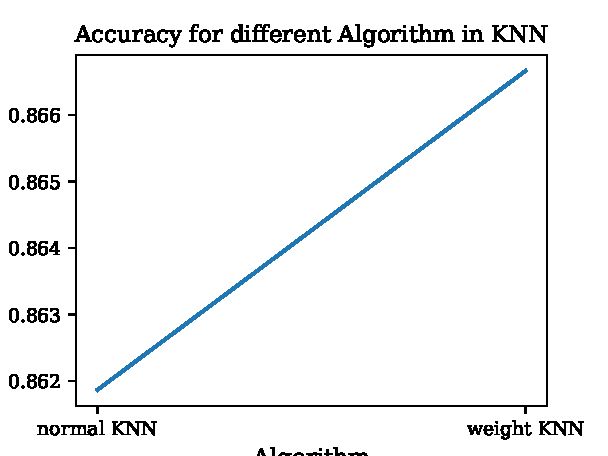
\includegraphics{figures/1h_knn_acc_algo.pdf}

We find very small increment in accuracy with Weight KNN.

\subsection{Misclassified samples}

As the task sheet required, for at least three different distance measures and features obtained from two different filters, we plot the nearest neighbors to 5 random misclassifed samples. To fulfill the requirement, we plot 3 different cases.

The first case is with a classifier with Euclidean distance metric and blur filter:

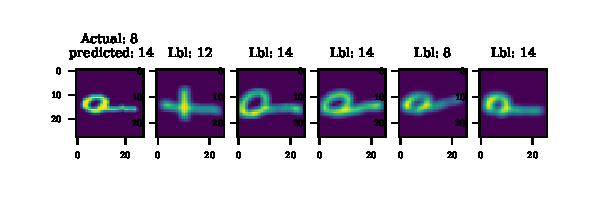
\includegraphics{figures/1i[1]_miss_classified_0.pdf}

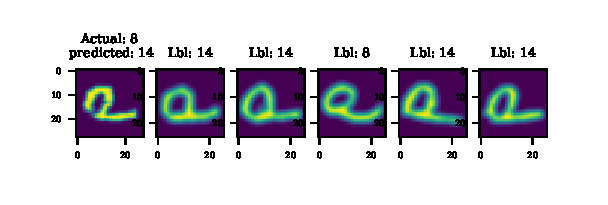
\includegraphics{figures/1i[1]_miss_classified_1.pdf}

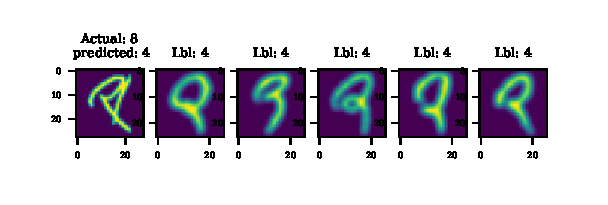
\includegraphics{figures/1i[1]_miss_classified_2.pdf}

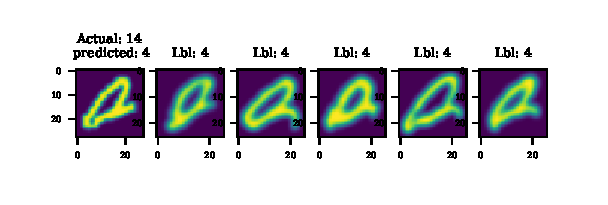
\includegraphics{figures/1i[1]_miss_classified_3.pdf}

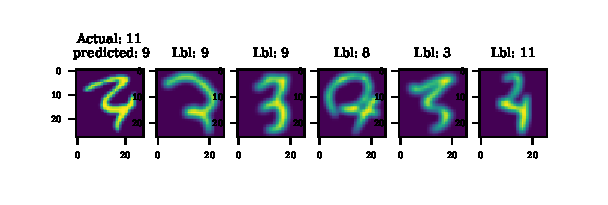
\includegraphics{figures/1i[1]_miss_classified_4.pdf}

The second case is with a classifier with Manhattan distance metric and blur filter:

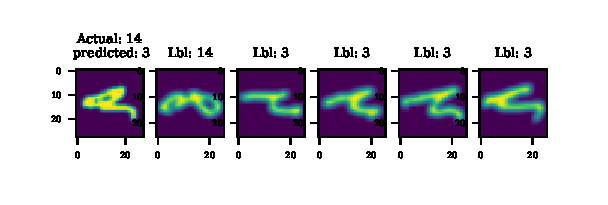
\includegraphics{figures/1i[2]_miss_classified_0.pdf}

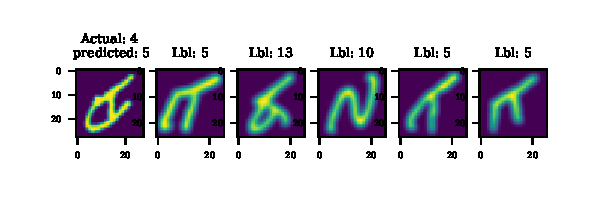
\includegraphics{figures/1i[2]_miss_classified_1.pdf}

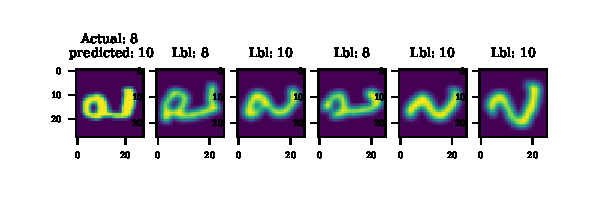
\includegraphics{figures/1i[2]_miss_classified_2.pdf}

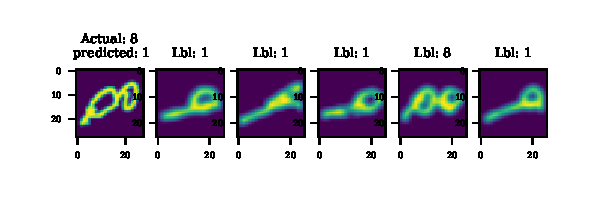
\includegraphics{figures/1i[2]_miss_classified_3.pdf}

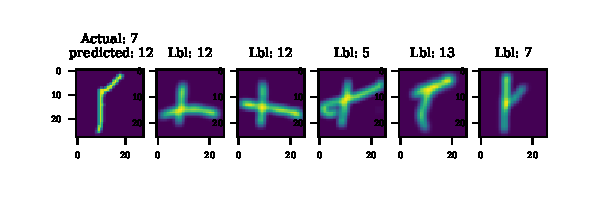
\includegraphics{figures/1i[2]_miss_classified_4.pdf}

The third case is with a classifier with Manhattan distance metric and edge filter:

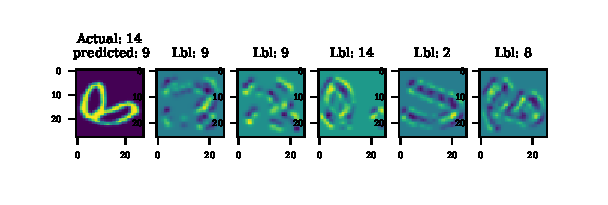
\includegraphics{figures/1i[3]_miss_classified_0.pdf}

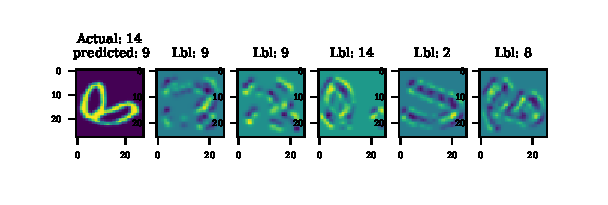
\includegraphics{figures/1i[3]_miss_classified_0.pdf}

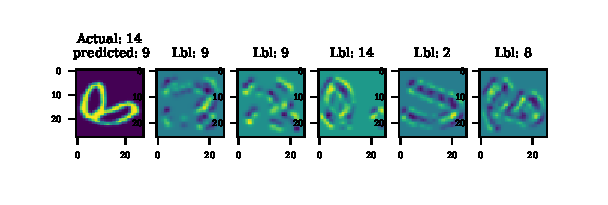
\includegraphics{figures/1i[3]_miss_classified_0.pdf}

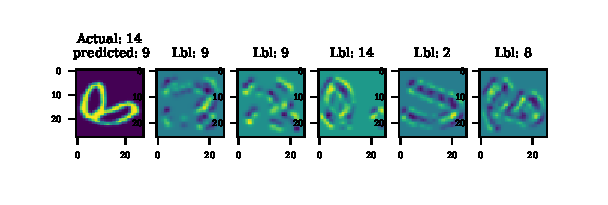
\includegraphics{figures/1i[3]_miss_classified_0.pdf}

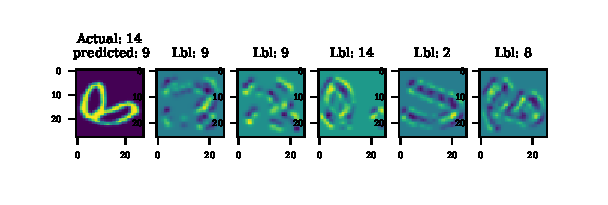
\includegraphics{figures/1i[3]_miss_classified_0.pdf}

Many misclassified images has a very close pattern compare to their neighbors but the result of the predictions are still incorrect. Because we have many images of different classes that look identical to each other, many was predicted with the wrong label.

\section{Deep Neural Network}
\subsection{Neural Network Term}

Before implementing, we need to present some definitions related to neural network.
\begin{itemize}
    \item Activation function: Activation functions define the output of each neuron in the network, they help the network use the important information and suppress the irrelevant data points, given (set of) input. Some of the functions are Sigmoid, ReLU
    \item Loss function: Loss function is the function that calculate the prediction error of the model, such as Mean Square Error, Cross Entropy...
    \item Parameter is specifications from the model, which can be estimated from the data (e.g. weight, bias). Hyper-parameter is specifications that there are no clear way to optimize and need to manually changed to find the best values. (e.g. k in KNN classifier, learning rate,...)
    \item Optimizer: Algorithm/Method, combined with a loss function, used to update the parameters of the network (for examples: weight, bias) in order to minimize that loss function. Examples of optimizers are Adam, Stochatical Gradient Descent...
    \item Epoch: Training all the given data in one cycle.
    \item Over-fitting: an error that occurs when a function is too closely aligned to a limited set of data points. As a result, the model is useful in reference only to its initial data set, and not to any other data sets. And underfitting is just the reversed way of overfitting.
    \item Training set: Training set is a set a data, which is used to train a model. Normally given as a pair of input and the actual output.
    \item Test set: Test set is a set of data, which is used to test how good (accurate) the current model is.
    \item Validation set: Validation set is a set of data which is used to tune the hyper-parameters of the model.
\end{itemize}

\subsection{Implementing Deep Neural Network}

As for the given task we implemented a linear neural network (layer: 784, 256, 64, 15).

\begin{itemize}
    \item learning\_rate = 0.001
    \item batch\_size = 128
    \item num\_epoch = 10
    \item Loss function: Cross Entropy
    \item Optimizer: Adam
\end{itemize}

\subsection{Changing Architecture Specification}

As we found our best number of layers and neurons for each layer. We compare our current CNN with another but with different loss function.

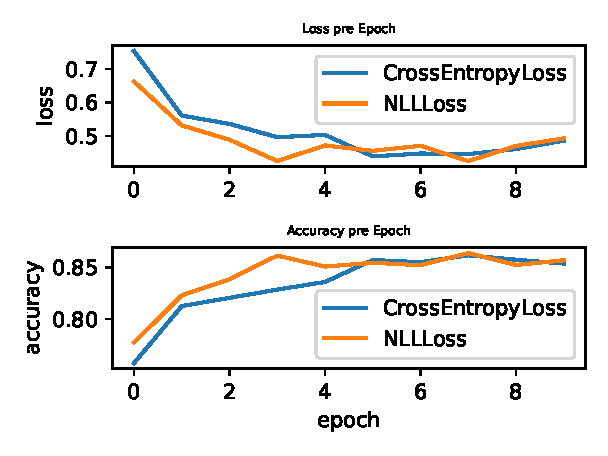
\includegraphics{figures/2c[1]_dnn_loss_epoch.pdf}

After 8 epochs, the accuracy of each model peaks and close to each other.

\subsection{Confusion Matrix and Confidence}

Confusion Matrix for our current CNN

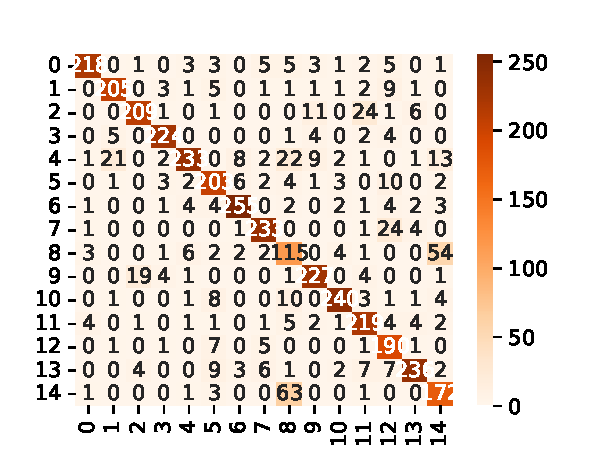
\includegraphics{figures/2d_confusion_matrix.pdf}

10 most unconfident each class:

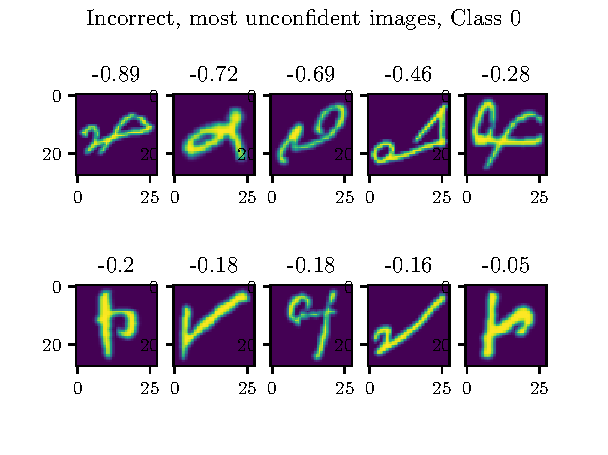
\includegraphics{figures/2d_unconfident_imgs_class_0.pdf}

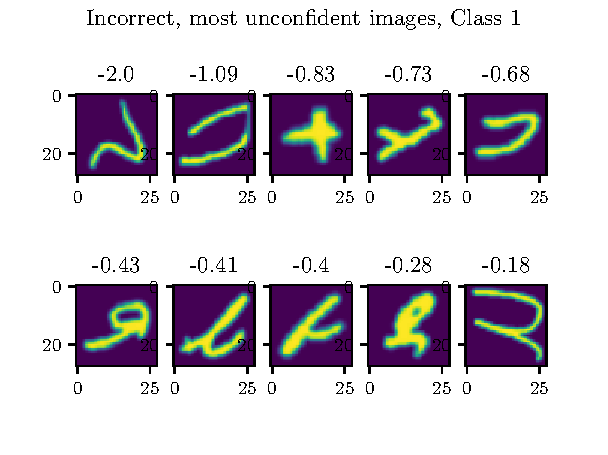
\includegraphics{figures/2d_unconfident_imgs_class_1.pdf}

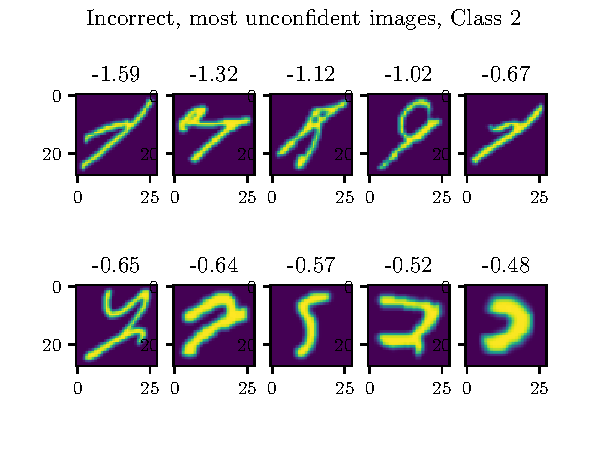
\includegraphics{figures/2d_unconfident_imgs_class_2.pdf}

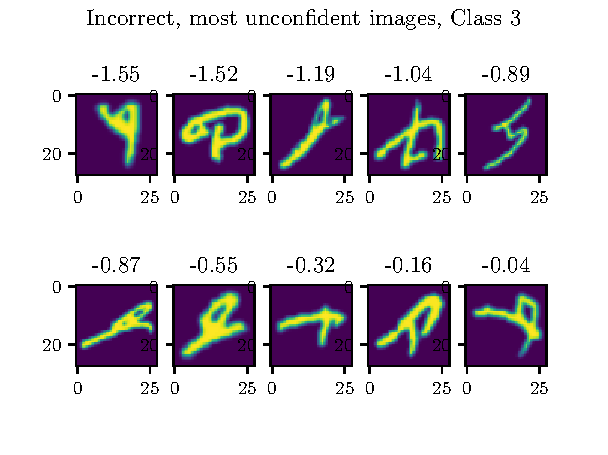
\includegraphics{figures/2d_unconfident_imgs_class_3.pdf}

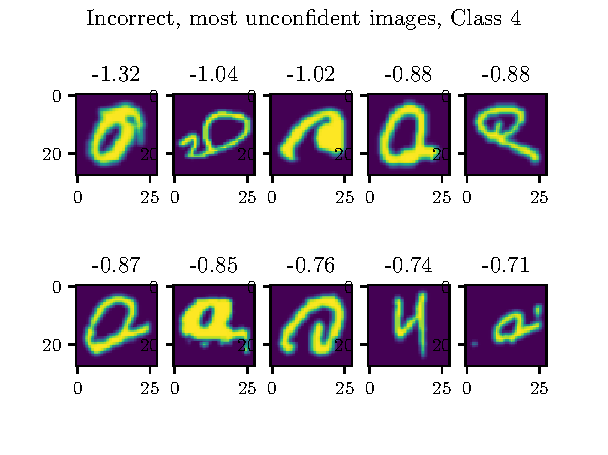
\includegraphics{figures/2d_unconfident_imgs_class_4.pdf}

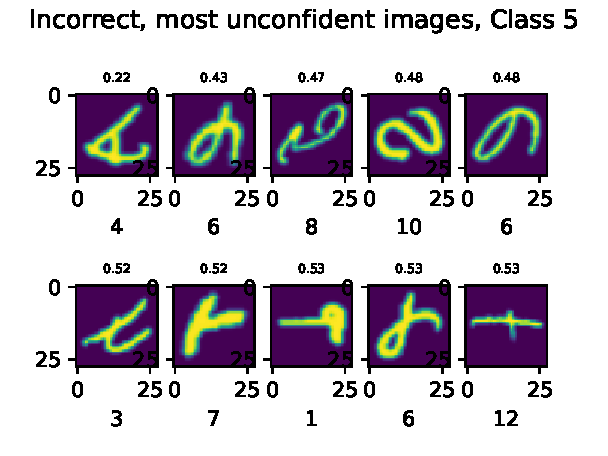
\includegraphics{figures/2d_unconfident_imgs_class_5.pdf}

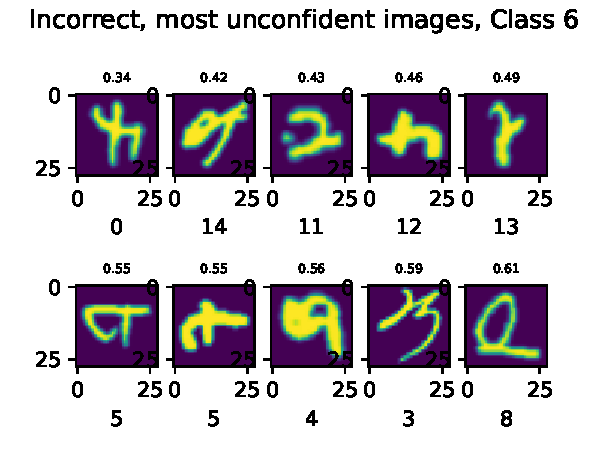
\includegraphics{figures/2d_unconfident_imgs_class_6.pdf}

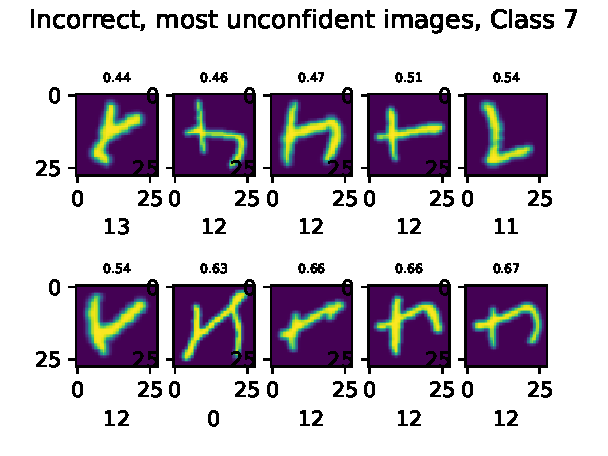
\includegraphics{figures/2d_unconfident_imgs_class_7.pdf}

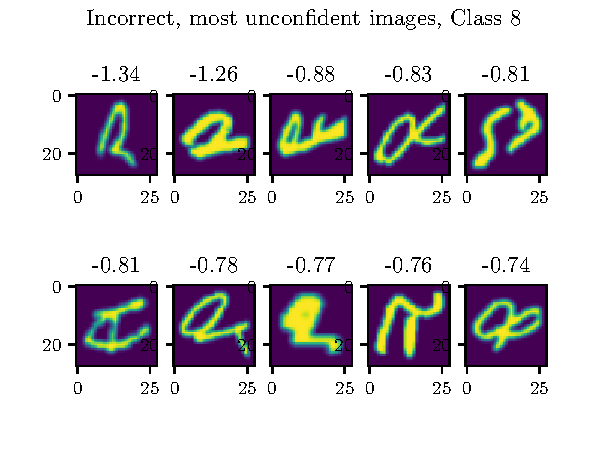
\includegraphics{figures/2d_unconfident_imgs_class_8.pdf}

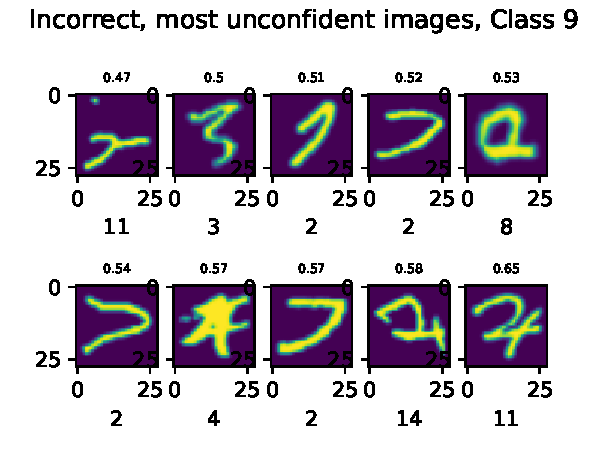
\includegraphics{figures/2d_unconfident_imgs_class_9.pdf}

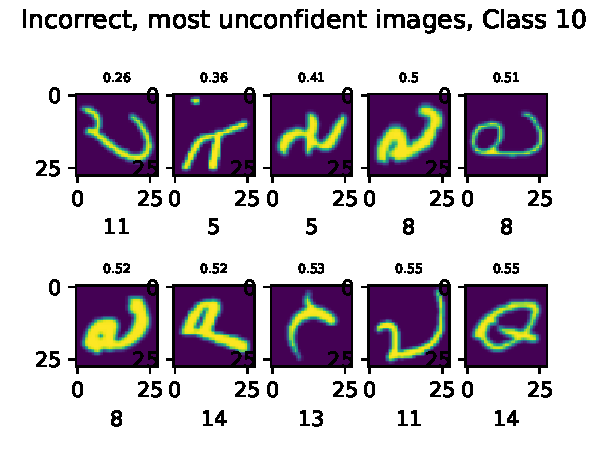
\includegraphics{figures/2d_unconfident_imgs_class_10.pdf}

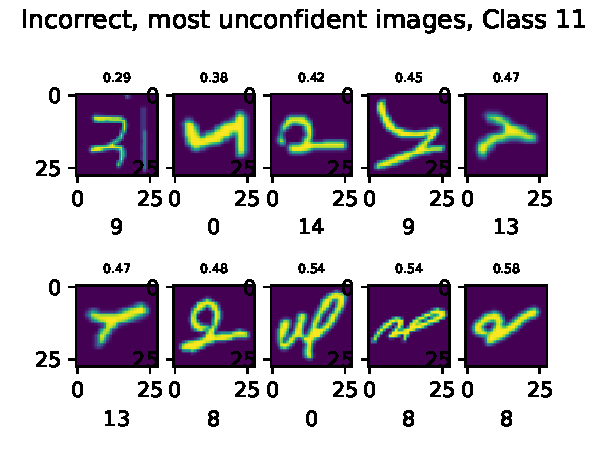
\includegraphics{figures/2d_unconfident_imgs_class_11.pdf}

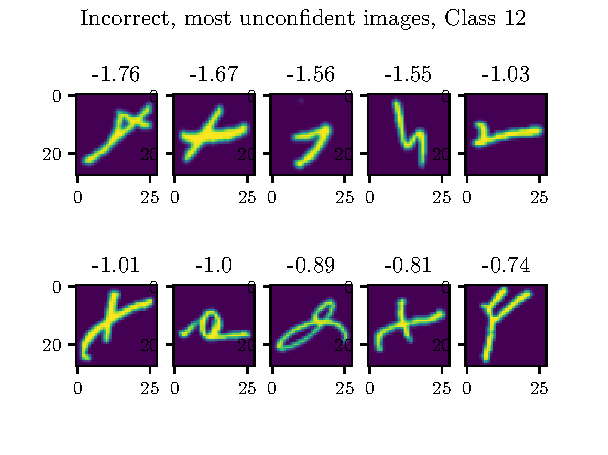
\includegraphics{figures/2d_unconfident_imgs_class_12.pdf}

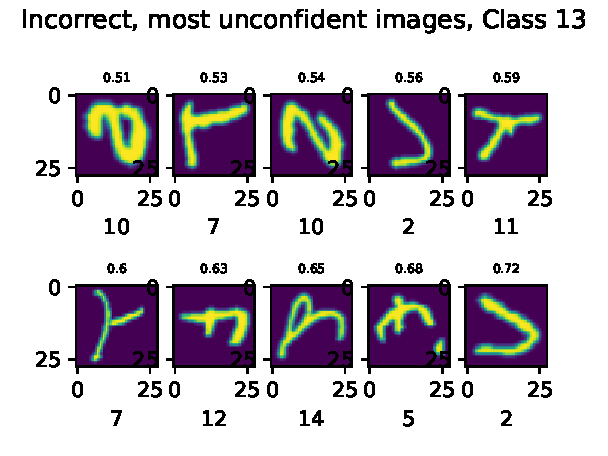
\includegraphics{figures/2d_unconfident_imgs_class_13.pdf}

\includegraphics{figures/2d_unconfident_imgs_class_14.pdf}

10 most confident each class:

\includegraphics{figures/2d_confident_imgs_class_0.pdf}

\includegraphics{figures/2d_confident_imgs_class_1.pdf}

\includegraphics{figures/2d_confident_imgs_class_2.pdf}

\includegraphics{figures/2d_confident_imgs_class_3.pdf}

\includegraphics{figures/2d_confident_imgs_class_4.pdf}

\includegraphics{figures/2d_confident_imgs_class_5.pdf}

\includegraphics{figures/2d_confident_imgs_class_6.pdf}

\includegraphics{figures/2d_confident_imgs_class_7.pdf}

\includegraphics{figures/2d_confident_imgs_class_8.pdf}

\includegraphics{figures/2d_confident_imgs_class_9.pdf}

\includegraphics{figures/2d_confident_imgs_class_10.pdf}

\includegraphics{figures/2d_confident_imgs_class_11.pdf}

\includegraphics{figures/2d_confident_imgs_class_12.pdf}

\includegraphics{figures/2d_confident_imgs_class_13.pdf}

\includegraphics{figures/2d_confident_imgs_class_14.pdf}

As expected, for unconfident images in each class, they does not look identical or share a common pattern with each other. The opposite applies for confident images.

\subsection{KNN Version}

In this task, we run both normal and KNN versions with 4-fold validation. The accuracy of KNN version is just 1\% higher, but way more costly than the normal, since the KNN runs extremely slow by large dadasets. 

\includegraphics{figures/2e_dnn.pdf}

\subsection{Batch Normalization}

Batch Normalization is implemented as follows:
\begin{lstlisting}[language=python]
class BatchNorm(nn.Module):
        def __init__(self, C, momentum=0.9):
            super().__init__()
            self.C = C
            self.momentum=momentum
            self.running_mean = torch.zeros(C)
            self.running_var = torch.ones(C)
            self.weight = nn.Parameter(torch.randn(C)/math.sqrt(C))
            self.bias = nn.Parameter(torch.zeros(C))

        def forward(self, X):
            if self.training:
                mean = X.mean([0,2,3])
                var = X.var([0,2,3])
                self.running_mean = self.running_mean*self.momentum + mean*(1-self.momentum)
                self.running_var = self.running_var*self.momentum + var*(1-self.momentum)
            else:
                mean = self.running_mean
                var = self.running_var

            m = mean.view([1, self.C, 1, 1]).expand_as(X)
            v = var.view([1, self.C, 1, 1]).expand_as(X)
            w = self.weight.view([1, self.C, 1, 1]).expand_as(X)
            b = self.bias.view([1, self.C, 1, 1]).expand_as(X)
            out = w * (X - m)/torch.sqrt(v) + b
            return out
\end{lstlisting}

There is no hug differences when Batch Normalization is applied. We put a Batch Normalization layer before each Convolution layer.

\includegraphics{figures/2f_dnn.pdf}


% Print references
\end{document}